\documentclass{article}
\usepackage[paperwidth=220mm,paperheight=90mm,margin=4mm,noheadfoot]{geometry}
\usepackage{amsmath,amssymb}
\usepackage{helvet}
\usepackage{tikz}
\renewcommand{\familydefault}{\sfdefault}
\usetikzlibrary{arrows.meta,backgrounds,calc,fit,positioning,shapes.geometric}

% Okabe--Ito / Color Universal Design palette.  Colour is deliberately
% redundant with line style and shape so the workflow remains legible in grey.
\definecolor{ink}{HTML}{333333}
\definecolor{muted}{HTML}{5C6B73}
\definecolor{hair}{HTML}{A7B0B5}
\definecolor{blue}{HTML}{0072B2}
\definecolor{bluefill}{HTML}{F2F8FB}
\definecolor{vermillion}{HTML}{D55E00}
\definecolor{green}{HTML}{009E73}

\tikzset{
  every node/.style={text=ink},
  block/.style={draw=hair, fill=white, rounded corners=1.6pt,
    line width=.72pt, align=center, inner xsep=4pt, inner ysep=3pt,
    font=\fontsize{10.2}{11.4}\selectfont},
  llm/.style={block, draw=vermillion, line width=1.0pt},
  sub/.style={block, draw=blue, minimum height=14mm, line width=.85pt},
  simulator/.style={block, draw=green, minimum height=22mm, line width=1.0pt},
  mainflow/.style={-{Latex[length=2.4mm,width=1.45mm]}, draw=ink,
    line width=1.0pt},
  context/.style={-{Latex[length=2.1mm,width=1.25mm]}, draw=muted,
    densely dotted, line width=.82pt},
  knowledge/.style={-{Latex[length=2.4mm,width=1.45mm]}, draw=vermillion,
    dashed, line width=1.0pt},
  flowlabel/.style={font=\fontsize{8.7}{9.7}\selectfont, text=muted,
    fill=white, inner sep=1.1pt, align=center},
  boTitle/.style={font=\fontsize{9.3}{10.3}\selectfont\bfseries,
    text=blue, fill=bluefill, inner sep=1pt}
}

\begin{document}
\thispagestyle{empty}
\noindent
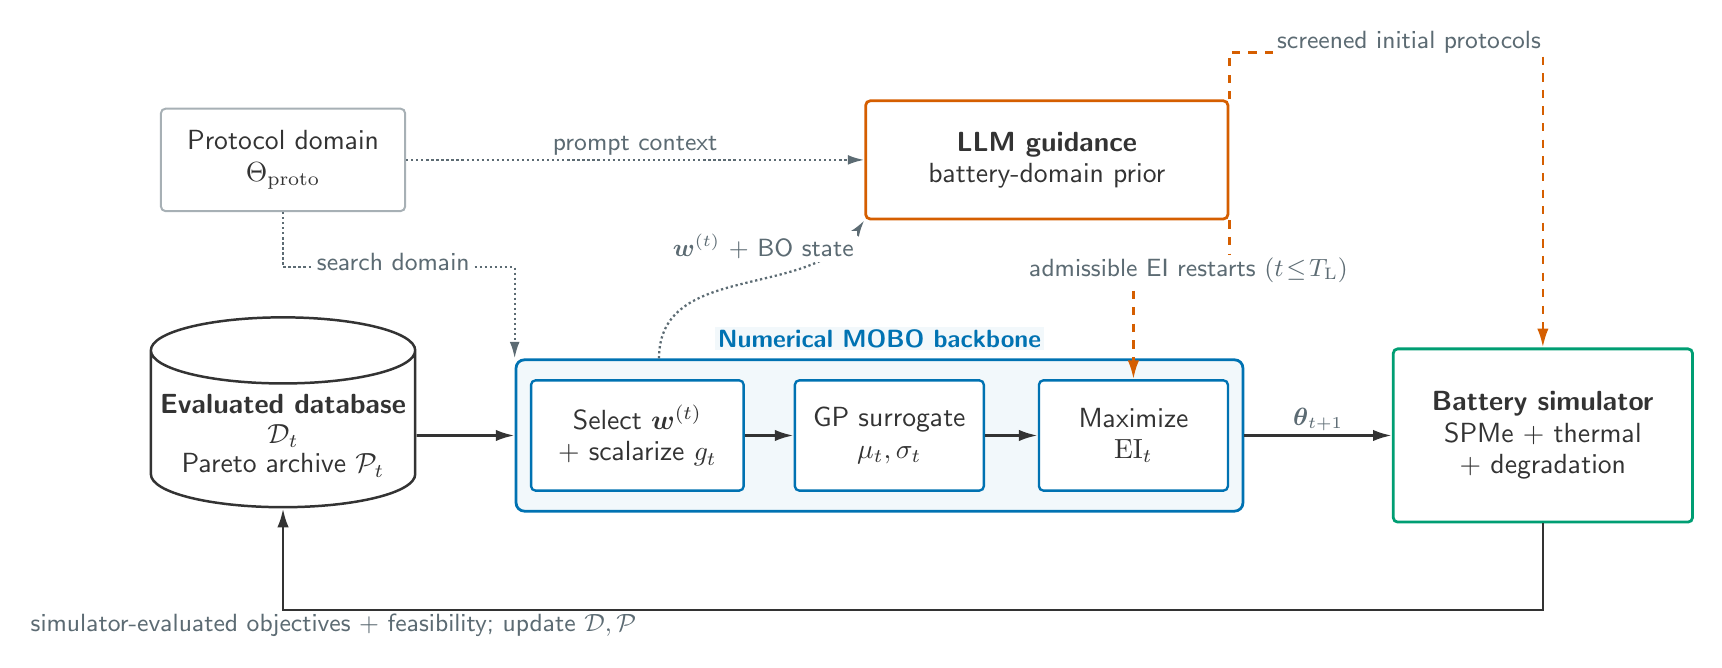
\begin{tikzpicture}[x=1mm,y=1mm]

% Shared protocol definition.  It conditions both the LLM prompt and the
% numerical optimizer; neither branch is allowed to redefine the domain.
\node[block, minimum width=31mm, minimum height=13mm] (domain) at (21,60)
  {Protocol domain\\$\Theta_{\mathrm{proto}}$};

\node[llm, minimum width=46mm, minimum height=15mm] (llm) at (118,60)
  {\textbf{LLM guidance}\\battery-domain prior};

% Evaluated information is neutral: it is the state consumed by the numerical
% loop, not a third algorithmic branch.
\node[shape=cylinder, shape border rotate=90, aspect=.25,
  draw=ink, fill=white, line width=.9pt,
  minimum width=27mm, minimum height=22mm,
  font=\fontsize{9.8}{10.8}\selectfont, align=center] (data) at (21,25)
  {\textbf{Evaluated database}\\$\mathcal D_t$\\Pareto archive $\mathcal P_t$};

% Numerical backbone, matching the algorithmic order in the paper.
\node[sub, minimum width=27mm] (scalar) at (66,25)
  {Select $\boldsymbol w^{(t)}$\\+ scalarize $g_t$};
\node[sub, minimum width=24mm] (gp) at (98,25)
  {GP surrogate\\$\mu_t,\sigma_t$};
\node[sub, minimum width=24mm] (ei) at (129,25)
  {Maximize\\$\mathrm{EI}_t$};

\draw[mainflow] (scalar) -- (gp);
\draw[mainflow] (gp) -- (ei);

\begin{scope}[on background layer]
  \node[draw=blue, fill=bluefill, rounded corners=3pt, line width=1.0pt,
    fit=(scalar)(gp)(ei), inner xsep=5pt, inner ysep=7pt] (mobo) {};
\end{scope}
\node[boTitle, anchor=south] at ([yshift=1.0mm]mobo.north)
  {Numerical MOBO backbone};

% Physical oracle.  Both initial and sequential protocols enter this same gate.
\node[simulator, minimum width=38mm] (sim) at (181,25)
  {\textbf{Battery simulator}\\SPMe + thermal\\+ degradation};

% Full-budget numerical loop.
\draw[mainflow] (data) -- (mobo);
\draw[mainflow] (mobo) --
  node[flowlabel,above]{$\boldsymbol\theta_{t+1}$} (sim);
\draw[mainflow] (sim.south) -- ++(0,-11) -|
  node[flowlabel,pos=.48,below]
  {simulator-evaluated objectives + feasibility; update $\mathcal D,\mathcal P$}
  (data.south);

% The domain is shared by both search mechanisms.
\draw[context] (domain.east) --
  node[flowlabel,above]{prompt context} (llm.west);
\draw[context] (domain.south) -- ++(0,-7) -| (mobo.north west);
\node[flowlabel] at (35,47.0) {search domain};

% Online regional guidance is explicitly conditioned on the current numerical
% state.  Input and output use different anchors so their directions are clear.
\draw[context] ([xshift=-28mm]mobo.north) to[out=90,in=235]
  (llm.south west);
\node[flowlabel] at (82,49.0) {$\boldsymbol w^{(t)}$ + BO state};
\draw[knowledge] (llm.south east) -- ++(0,-7) -| (ei.north);
\node[flowlabel] at (136,46.0)
  {admissible EI restarts $(t\!\leq\!T_{\mathrm L})$};

% Warm-start proposals go to the simulator, never directly to the database.
\draw[knowledge] (llm.north east) -- ++(0,6) -| (sim.north);
\node[flowlabel] at (164,75.0) {screened initial protocols};

\end{tikzpicture}
\end{document}
